\documentclass[dvipdfmx]{jarticle}
\usepackage{graphicx}
\usepackage[top=30truemm,bottom=30truemm,left=25truemm,right=25truemm]{geometry}
\usepackage{listings,jvlisting}
\usepackage{url}

\lstset{
  basicstyle={\ttfamily},
  identifierstyle={\small},
  commentstyle={\smallitshape},
  keywordstyle={\small\bfseries},
  ndkeywordstyle={\small},
  stringstyle={\small\ttfamily},
  frame={tb},
  breaklines=true,
  columns=[l]{fullflexible},
  numbers=left,
  xrightmargin=0zw,
  xleftmargin=3zw,
  numberstyle={\scriptsize},
  stepnumber=1,
  numbersep=1zw,
  lineskip=-0.5ex
}

\begin{document}
\begin{titlepage}
    \begin{center}
        {\huge 情報科学演習C 課題1レポ―ト}
        \vspace{180pt}\\
        \begin{tabular}{rl}
            氏名 & 山久保孝亮\\
            所属 & 大阪大学基礎工学部情報科学科ソフトウェア科学コース\\
            メールアドレス & u327468b@ecs.osaka-u.ac.jp\\
            学籍番号 & 09B22084\\
            提出日 & \today\\
            担当教員 & 平井健士 中島悠太
        \end{tabular}
    \end{center}
\end{titlepage}
\section{課題1-1}
\begin{enumerate}
    \item ping exp001を実行すると以下の図1のような出力結果が得られる.
    \begin{figure}[h]
        \centering
        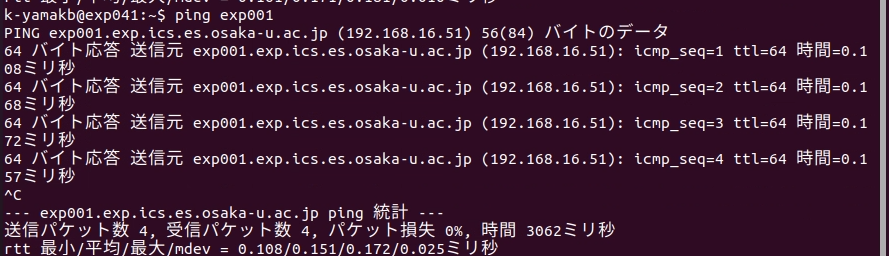
\includegraphics[width=14cm]{1-1-1.png}
        \caption{ping exp001の実行結果}
    \end{figure}
    \\pingコマンドはECHO\_REQUESTを使用してホストからECHO\_RESPONSEを引き出し、通信の状態を確認するコマンドである.ECHO\_REQUESTとECHO\_RESPONSEはICMPのメッセージである.
    1行目には左から順に,宛先として指定したサーバとそのIPアドレス,送信するパケットデータのサイズを表示している.56(84)は,56byteのデータにICMPのヘッダー情報の8byteとTCPデータの20byteが足されて合計84byteのデータが送信されるということを表している.
    2行目以降は同じ結果が繰り返し出力されている.繰り返されているそれぞれの内容は以下の通りである.
    \begin{itemize}
        \item 64バイト応答:送信されたICMPのデータサイズ(TCPのヘッダー情報の20byteは含まない)
        \item 送信元:宛先ホスト名とIPアドレス
        \item icmp\_seq:pingを送信した回数.この回数に抜けがあればその部分でパケットロスが発生している.
        \item ttl:パケットの生存期間.ネットワーク上でルータなどの危機を通過するたびにその値を1ずつ減らしていき,この値が0になるとパケットは破棄される
        \item 時間:パケットを送信して返ってくるまでの時間
    \end{itemize}
    そしてCtrl+Cを押して強制終了すると統計値が表示される.出力される内容は以下のとおりである.
    \begin{itemize}
        \item 送信パケット数:pingを送信した回数
        \item 受信パケット数:pingを送信してから宛先ホストから正常にパケットが戻ってきた回数
        \item パケット損失:送信パケットに対するパケットロスの割合
        \item 時間:pingを開始してから終了するまでにかかった時間
        \item rtt 最小/平均/最大/mdev:左から順に応答時間の最小値,平均値,最大値,標準誤差
    \end{itemize}
    \clearpage
    \item ドメインを入力した時もIPアドレスを入力したときも以下の図2のような同じ大阪大学のウェブサイトが開いた.
    \begin{figure}[h]
        \centering
        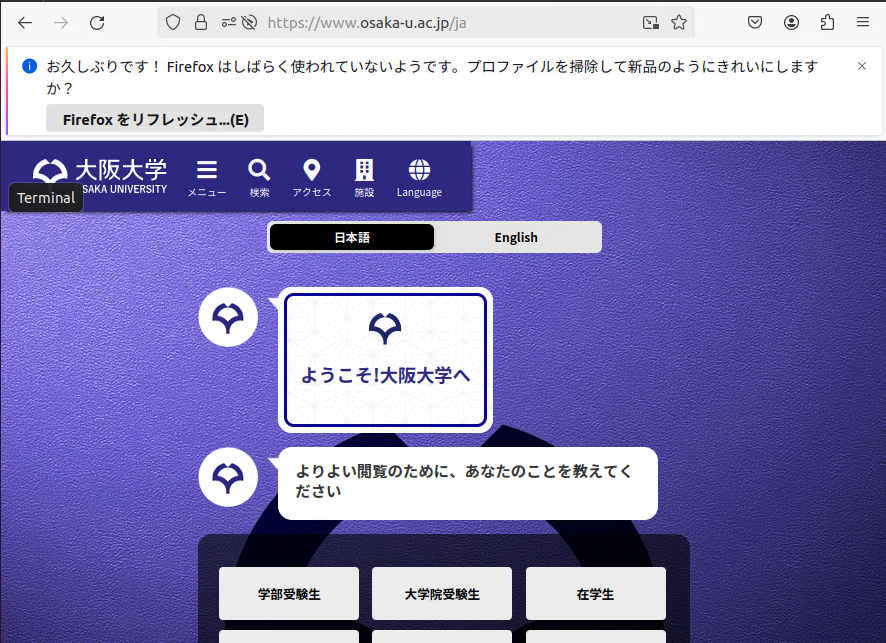
\includegraphics[width=8cm]{1-1-2.png}
        \caption{検索結果}
    \end{figure}
    このことから,www.osaka-u.ac.jpというドメインはIPアドレスに変換すると133.1.138.1となったと考えられる.
    \item nslookup osaka-u.ac.jpを実行すると以下の図3のような実行結果が得られる.
    \begin{figure}[h]
        \centering
        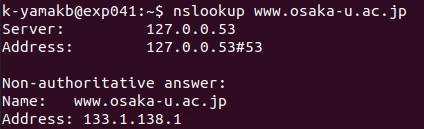
\includegraphics[width=12cm]{1-1-3.png}
        \caption{コマンドの実行結果}
    \end{figure}
    \\nslookupコマンドは二つのモードがあり,対話モードでは様々なホストやドメインに関する情報をネームサーバーに問い合わせたり、 ドメイン内のホストの一覧を表示したりすることができる.
    非対話モードではホストやドメインの名前と要求された情報だけを表示する.これによりドメイン名からIPアドレスを,IPアドレスからドメイン名を知ることができる.\\
    1.において,宛先ホスト名を指定したときにそれに対応するIPアドレスが表示されていた.このホスト名をnslookupコマンドを使ってIPアドレスを調べると以下の図4のようになる.
    \begin{figure}[h]
        \centering
        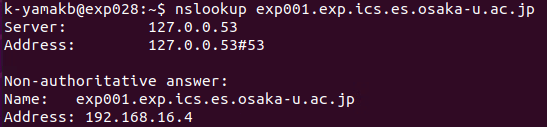
\includegraphics[width=12cm]{1-1-3-1.png}
        \caption{コマンドの実行結果}
    \end{figure}
    \\この出力結果から,Non-authoritative answerの方のアドレスとIPアドレスが一致していることがわかる.Non-authoritative answerは,キャッシュDNSから返ってきた情報であるということを表している.
    また,2.においてドメインとIPアドレスが同じであると考察したが,図3の出力結果からもそのことを確認することができる.
\end{enumerate}
\section{課題1-2}
\begin{enumerate}
    \setcounter{enumi}{3}
    \item /usr/sbin/arp -aを実行すると以下の図5のような出力が得られる.
    \begin{figure}[h]
        \centering
        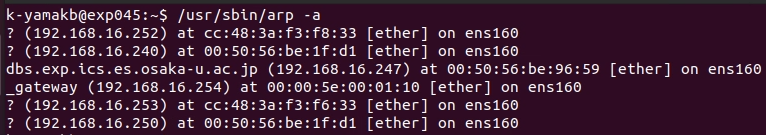
\includegraphics[width=12cm]{1-2-4.png}
        \caption{コマンドの実行結果}
    \end{figure}
    \\このコマンドによってARPキャッシュが出力として表示される.具体的な表示内容としては,まず最初にドメイン(IPアドレス)が表示され,その後atに続いてそれに対応するMACアドレスが表示される.
    [ether]というのはARPがIPアドレスをMACアドレスに変換する際にイーサネットフレーム内で動作するため表示されている.ens160というのはLinuxシステム上で特定のネットワークインターフェースを識別するための名前である.
    \item pingをexp002とexp003に対して実行すると以下の図6のような出力が得られた.
    \begin{figure}[h]
        \centering
        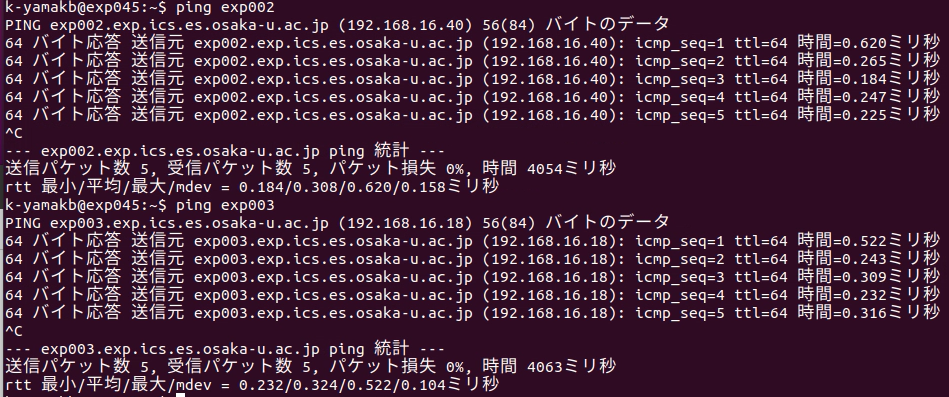
\includegraphics[width=12cm]{1-2-5.png}
        \caption{コマンドの実行結果}
    \end{figure}
    基本的な出力内容は上の1.で述べた内容と同じであったが,IPアドレスは異なっていた.
    以下の図7は図6の出力の後に/usr/sbin/arp -aを実行したときの出力である.
    \begin{figure}[h]
        \centering
        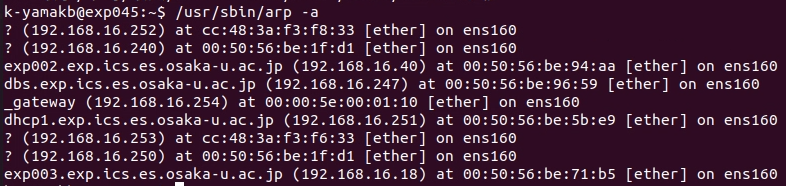
\includegraphics[width=12cm]{1-2-5-2.png}
        \caption{コマンドの実行結果}
    \end{figure}
    図5の出力結果と比べて,exp002とexp003のIPアドレスとMACアドレスのキャッシュが出力に追加されている.出力が変化した理由としては,pingコマンドによりメッセージのやり取りが行われたことで
    ARPキャッシュの内容が変化したためであると考えられる.
    \item /usr/sbin/tracerouteをexp002exp003,Webサーバ,ゲートウェイに対して実行すると以下の図8のような出力が得られる.
    \begin{figure}[h]
        \centering
        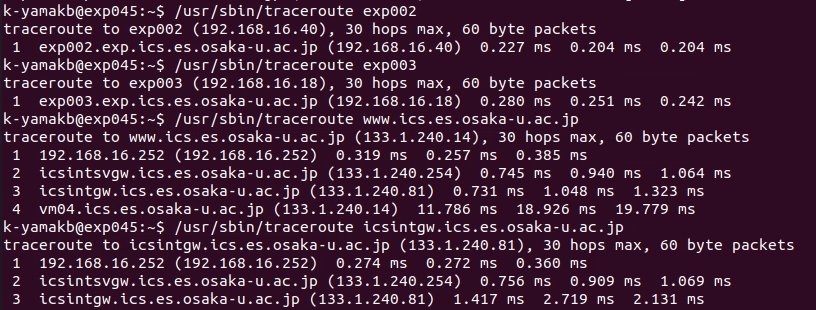
\includegraphics[width=12cm]{1-2-6.png}
        \caption{コマンドの実行結果}
    \end{figure}
    \\図8の出力結果を比較すると,exp002とexp003に対してtracerouteを実行したときは同じとなるがその二つとWebサーバ,ゲートウェイに対してtracerouteを
    実行したときには異なる結果となることがわかる.tracerouteコマンドは目的のIPアドレスまでの経路を表示するコマンドであり,それぞれ目的地のIPアドレスが異なるために
    出力の内容が異なると考えられる.
    \item pingとtracerouteが正しく動作することで宛先までのネットワーク経路と,その経路まで到達することが可能かどうかを知ることができる.つまり,exp001などのホストやWebサーバに対して先ほどの2つのコマンドが実行することによってネットワークの構成を予測することができる.
    今回推測したネットワークの構成は以下の図9のようになった.
    \begin{figure}[h]
        \centering
        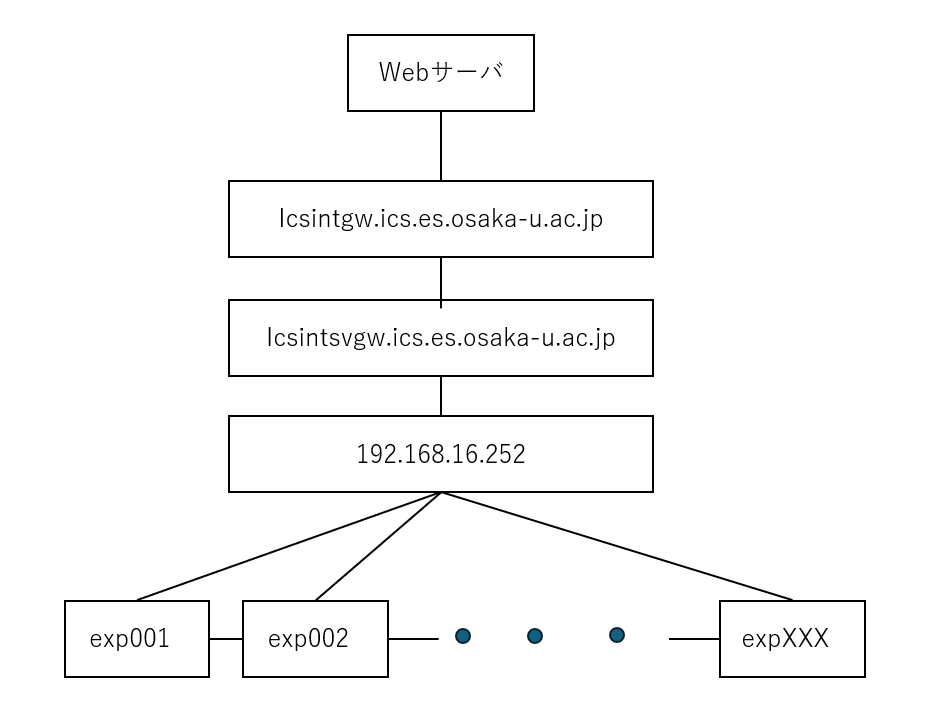
\includegraphics[width=12cm]{1-2-7.png}
        \caption{推測したネットワークの模式図}
    \end{figure}
    \\これは,図8におけるtracerouteコマンドの実行結果が,Webサーバに対して実行した際に,まず実際のIPアドレスである192.168.16.252を通りその後仮想IPアドレスである192.168.16.254を通ってからWebのドメインを通っていたことと,それぞれのホストに対して実行したときに
    一度の移動で到達することができていたことから,ホスト同士がつながっていると考えたためにこのような図となった.
    \item /bin/netstat -rを実行すると以下の図7のような実行結果が得られる.
    \begin{figure}[h]
        \centering
        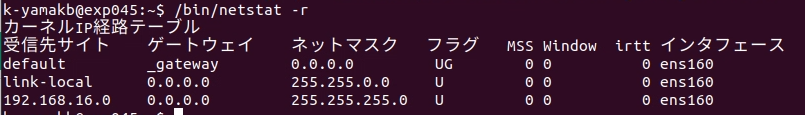
\includegraphics[width=14cm]{1-2-8.png}
        \caption{コマンドの実行結果}
    \end{figure}
    netstatはrオプションで実行するとルーティングテーブルを出力する.具体的な出力内容は以下のようになる.
    \begin{itemize}
        \item 受信先サイト:宛先のIPアドレス.
        \item ゲートウェイ:ゲートウェイのIPアドレス.
        \item ネットマスク:サブネットマスク.
        \item フラグ:Uは送信経路がリンクアップしていることを示し,Gは送信経路がゲートウェイ宛であることを示し,Hは宛先がネットワークではなく完全指定のホストアドレスであることを示している.
        \item MSS:Maximum Segment Sizeを表す.
        \item Window:TCP Window Sizeを表す.
        \item irtt:Initial Round Trip Timeを表す.
    \end{itemize}
    このことから,自分が想像したネットワークは
    \item 以下の図11は"ping exp001"を実行した直後に"/usr/sbin/arp -a"を実行したときの出力結果で,その下の図12は20分が経過した後に"/usr/sbin/arp -a"を実行したときの出力結果である.
    \begin{figure}[h]
        \centering
        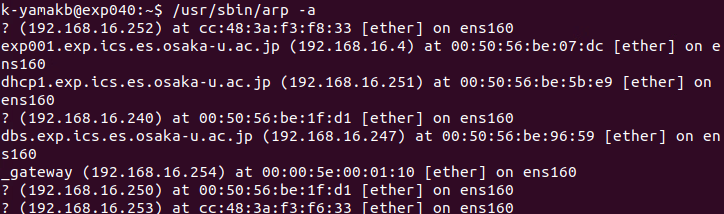
\includegraphics[width=8cm]{1-2-9-1.png}
        \caption{コマンドの実行結果}
    \end{figure}
    \begin{figure}[h]
        \centering
        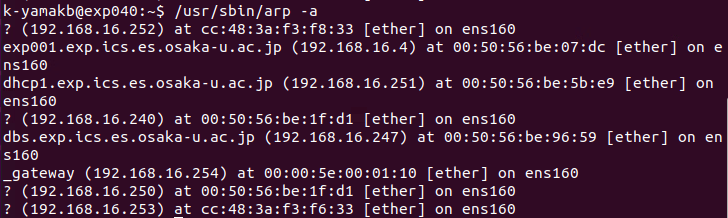
\includegraphics[width=8cm]{1-2-9-2.png}
        \caption{コマンドの実行結果}
    \end{figure}
    \\上の図11と12より,何も変化が起こらなかったことがわかる.Linuxのarpキャッシュは数分経てばキャッシュから追い出されて出力されなくなるはずであるが,何も変化が起こっていない.
    これの理由はARPキャッシュのタイムアウトの設定が長くなっているか,ARPリクエストがあまり行われないためにキャッシュが更新されないことなどが考えられる.
\end{enumerate}
\section{課題1-3}
\begin{enumerate}
\setcounter{enumi}{9}
    \item システムコールとは,カーネルとアプリケーションプログラムのインターフェースである.システムコールによってハードウェアの挙動を隠ぺいすることによってハードウェアによらずにデバイスからの入出力処理を行うことができるようになる.標準ライブラリ関数はあらかじめテストされているためコーディングの効率性と安定性が向上するという利点がある.
    ただし,
    また,標準ライブラリ関数とは,プログラミング言語の標準仕様に含まれる関数のことで,システムコールを利用するものも,利用しないものも存在する.ファイル処理に関して,システムコールは標準ライブラリ関数に比べて使いやすさや実行効率が劣ってしまうという欠点がある.
    しかし,ファイルの属性を変更するなどのシステムコールでしかできないような利点も存在するので,標準ライブラリ関数でfwriteとシステムコールのwriteのような同じような機能の仕組みが複数提供されている.ほかにもシステムコールでしかできないような
    例を挙げると,プログラムの実行中に新しいプロセスを生成したり,シグナルを送ったりするなどである.システムにとって重要で基幹部分に近いプログラムを作成したいときはシステムコールを使うことが必須となる.
    \item "strace -c echo hello"を実行すると以下の図13のような実行結果が得られる.
    \begin{figure}[h]
        \centering
        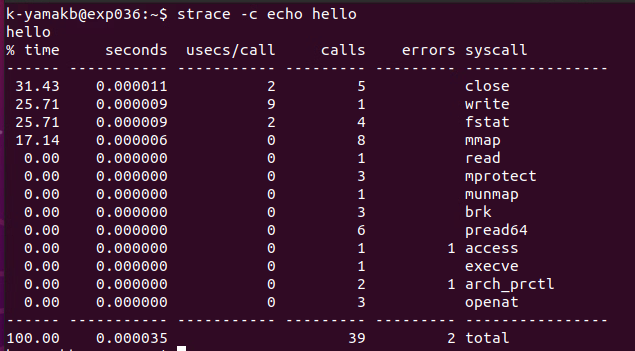
\includegraphics[width=8cm]{1-3-11.png}
        \caption{コマンドの実行結果}
    \end{figure}
    \\strace -cコマンドはシステムコールの数を取得することができる.出力は以下のようになると考えられる.
    \begin{itemize}
        \item \% time:各システムコールがプロセスを実行した時間のパーセント
        \item seconds:各システムコールが実行された合計時間
        \item usecs/call:各システムコールの平均実行時間
        \item calls:各システムコールが実行された回数
        \item errors:エラーが発生した場合のエラーコード
        \item syscall:実行されたシステムコールの名前
    \end{itemize}
    以下の図14はstrace -c lsを実行した結果である.
    \clearpage
    \begin{figure}[h]
        \centering
        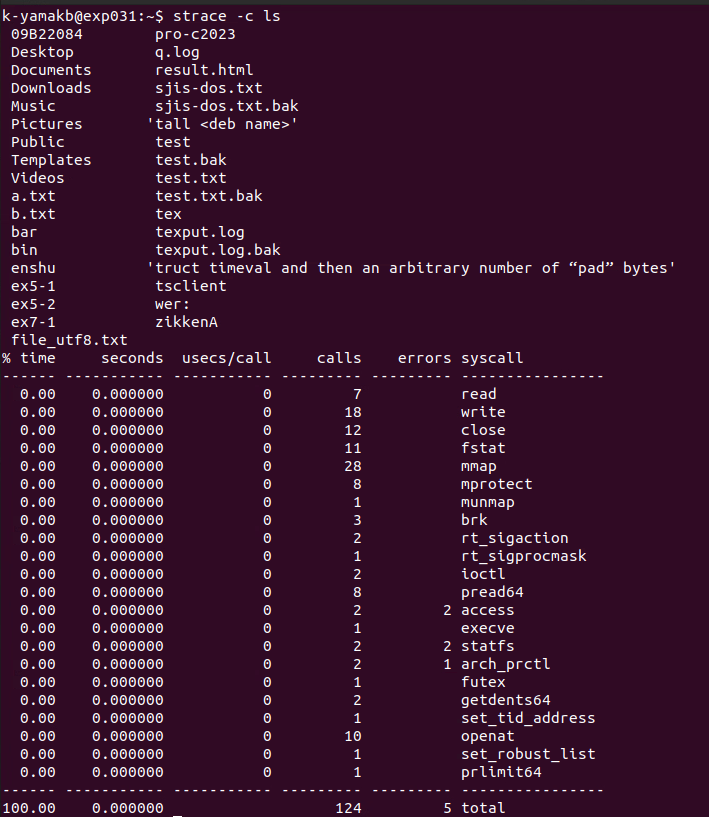
\includegraphics[width=8cm]{1-3-12-1.png}
        \caption{コマンドの実行結果}
    \end{figure}
    echoの時と比較して違う点は,システムコールの実行時間がほぼ全てゼロであるという点である.
\end{enumerate}
\section{感想}
今回の課題を通して,コマンドを使用してネットワーク上での通信の情報を取得したり,IPアドレスとドメインの関係,MACアドレス等について理解を深めることができた.ネットワーク関連の話題は学習意欲はあったがこれまで触れてきていなかったので,今後の課題においても
知識を身につける場であると考えて積極的に学習を進めていきたいと思う.また,システムコールについては,現在オペレーティングシステムの授業でカーネル等について学んでいるので,どこかで登場する機会がある考えられる知識を予め知ることができてよかったと感じた.
\section{謝辞}
今回の課題を通して質問対応,レポート採点等をしてくださった教授,TAの皆様方ありがとうございました.今後の課題もよろしくお願いいたします.
\section{参考文献}
\begin{itemize}
    \item \url{https://www.server-memo.net/tips/command/ping/ping.html#toc2} 4/28
    \item \url{https://win2012r2.com/2022/07/04/dns-non-authoritative-answer/} 4/28
    \item \url{https://www.oresamalabo.net/entry/2020/05/11/180603} 4/28
    \item \url{https://curtaincall.weblike.jp/portfolio-unix/api.html} 4/28
    \item \url{https://engineer-oasis.com/898/#} 4/28
    \item \url{https://relax-tech.net/linux-strace-debug/#rtoc-7} 4/28
\end{itemize}
\end{document}